%% BioMed_Central_Tex_Template_v1.06
%%                                      %
%  bmc_article.tex            ver: 1.06 %
%                                       %

%%IMPORTANT: do not delete the first line of this template
%%It must be present to enable the BMC Submission system to
%%recognise this template!!

%%%%%%%%%%%%%%%%%%%%%%%%%%%%%%%%%%%%%%%%%
%%                                     %%
%%  LaTeX template for BioMed Central  %%
%%     journal article submissions     %%
%%                                     %%
%%          <8 June 2012>              %%
%%                                     %%
%%                                     %%
%%%%%%%%%%%%%%%%%%%%%%%%%%%%%%%%%%%%%%%%%

%%%%%%%%%%%%%%%%%%%%%%%%%%%%%%%%%%%%%%%%%%%%%%%%%%%%%%%%%%%%%%%%%%%%%
%%                                                                 %%
%% For instructions on how to fill out this Tex template           %%
%% document please refer to Readme.html and the instructions for   %%
%% authors page on the biomed central website                      %%
%% https://www.biomedcentral.com/getpublished                      %%
%%                                                                 %%
%% Please do not use \input{...} to include other tex files.       %%
%% Submit your LaTeX manuscript as one .tex document.              %%
%%                                                                 %%
%% All additional figures and files should be attached             %%
%% separately and not embedded in the \TeX\ document itself.       %%
%%                                                                 %%
%% BioMed Central currently use the MikTex distribution of         %%
%% TeX for Windows) of TeX and LaTeX.  This is available from      %%
%% https://miktex.org/                                             %%
%%                                                                 %%
%%%%%%%%%%%%%%%%%%%%%%%%%%%%%%%%%%%%%%%%%%%%%%%%%%%%%%%%%%%%%%%%%%%%%

%%% additional documentclass options:
%  [doublespacing]
%  [linenumbers]   - put the line numbers on margins

%%% loading packages, author definitions

%\documentclass[twocolumn]{bmcart}% uncomment this for twocolumn layout and comment line below
\documentclass{bmcart}

%%% Load packages
\usepackage{amsthm,amsmath}
\usepackage{tabularx}
\usepackage{xspace}
\usepackage{color}
\usepackage{epsfig}
\usepackage{caption}
\usepackage{subcaption}
\usepackage{mathrsfs}
\usepackage{amssymb}
\usepackage{amsmath}
\usepackage{amsthm}

\usepackage{tikz}
%\usepackage{fullpage}
\usepackage{calc}
\usetikzlibrary{positioning,shadows,arrows,trees,shapes,fit}
\usepackage{blindtext}
\usepackage{pgfplots}
%\pgfplotsset{compat=1.16}
\usepackage{pythonhighlight}
\usepackage{fixme}
\fxsetup{status=draft} % <====== add this line
\usepackage{mathtools}
\usepackage{algorithm}
\usepackage{algpseudocode}
  
\usepackage{url}
\raggedbottom
%\algnewcommand\algorithmicforeach{\textbf{for each}}
%\algdef{S}[FOR]{ForEach}[1]{\algorithmicforeach\ #1\ \algorithmicdo}

% scaling factor for tables
\newcommand\tabscale{0.8}
\newtheorem{definition}{Definition}
\newtheorem{Lemma}{Lemma}


\usepackage{fixme}

  
%\RequirePackage[numbers]{natbib}
%\RequirePackage[authoryear]{natbib}% uncomment this for author-year bibliography
%\RequirePackage{hyperref}
\usepackage[utf8]{inputenc} %unicode support
%\usepackage[applemac]{inputenc} %applemac support if unicode package fails
%\usepackage[latin1]{inputenc} %UNIX support if unicode package fails

%%%%%%%%%%%%%%%%%%%%%%%%%%%%%%%%%%%%%%%%%%%%%%%%%
%%                                             %%
%%  If you wish to display your graphics for   %%
%%  your own use using includegraphic or       %%
%%  includegraphics, then comment out the      %%
%%  following two lines of code.               %%
%%  NB: These line *must* be included when     %%
%%  submitting to BMC.                         %%
%%  All figure files must be submitted as      %%
%%  separate graphics through the BMC          %%
%%  submission process, not included in the    %%
%%  submitted article.                         %%
%%                                             %%
%%%%%%%%%%%%%%%%%%%%%%%%%%%%%%%%%%%%%%%%%%%%%%%%%

%\def\includegraphic{}
%\def\includegraphics{}

%%% Put your definitions there:
\startlocaldefs
\endlocaldefs

%%% Begin ...
\begin{document}

%%% Start of article front matter
\begin{frontmatter}

\begin{fmbox}
\dochead{Research}

%%%%%%%%%%%%%%%%%%%%%%%%%%%%%%%%%%%%%%%%%%%%%%
%%                                          %%
%% Enter the title of your article here     %%
%%                                          %%
%%%%%%%%%%%%%%%%%%%%%%%%%%%%%%%%%%%%%%%%%%%%%%

\title{Symbolic classification with RILS-ROLS and HROCH algorithms}

%%%%%%%%%%%%%%%%%%%%%%%%%%%%%%%%%%%%%%%%%%%%%%
%%                                          %%
%% Enter the authors here                   %%
%%                                          %%
%% Specify information, if available,       %%
%% in the form:                             %%
%%   <key>={<id1>,<id2>}                    %%
%%   <key>=                                 %%
%% Comment or delete the keys which are     %%
%% not used. Repeat \author command as much %%
%% as required.                             %%
%%                                          %%
%%%%%%%%%%%%%%%%%%%%%%%%%%%%%%%%%%%%%%%%%%%%%%

\author[
  addressref={aff1},                   % id's of addresses, e.g. {aff1,aff2}
  corref={aff1},                       % id of corresponding address, if any
% noteref={n1},                        % id's of article notes, if any
  email={kartelj@matf.bg.ac.rs}   % email address
]{\inits{A.K.}\fnm{Aleksandar} \snm{Kartelj}}
\author[
  addressref={aff2},
  email={marko.djukanovic@pmf.unibl.org}
]{\inits{M.DJ.}\fnm{Marko} \snm{Djukanović}}

\author[
email={jan.pigos@gmail.com}
]{\inits{M.DJ.}\fnm{Jan} \snm{Pingos}}

%%%%%%%%%%%%%%%%%%%%%%%%%%%%%%%%%%%%%%%%%%%%%%
%%                                          %%
%% Enter the authors' addresses here        %%
%%                                          %%
%% Repeat \address commands as much as      %%
%% required.                                %%
%%                                          %%
%%%%%%%%%%%%%%%%%%%%%%%%%%%%%%%%%%%%%%%%%%%%%%

\address[id=aff1]{%                           % unique id
  \orgdiv{Department of Informatics, Faculty of Mathematics},             % department, if any
  \orgname{University of Belgrade},          % university, etc
  \city{Belgrade},                              % city
  \cny{Serbia}                                    % country
}
\address[id=aff2]{%
  \orgdiv{Faculty of Sciences and Mathematics},
  \orgname{University of Banja Luka},
  %\street{},
  %\postcode{}
  \city{Banja Luka},
  \cny{Bosnia and Herzegovina}
}

%%%%%%%%%%%%%%%%%%%%%%%%%%%%%%%%%%%%%%%%%%%%%%
%%                                          %%
%% Enter short notes here                   %%
%%                                          %%
%% Short notes will be after addresses      %%
%% on first page.                           %%
%%                                          %%
%%%%%%%%%%%%%%%%%%%%%%%%%%%%%%%%%%%%%%%%%%%%%%

%\begin{artnotes}
%%\note{Sample of title note}     % note to the article
%\note[id=n1]{Equal contributor} % note, connected to author
%\end{artnotes}

\end{fmbox}% comment this for two column layout

%%%%%%%%%%%%%%%%%%%%%%%%%%%%%%%%%%%%%%%%%%%%%%%
%%                                           %%
%% The Abstract begins here                  %%
%%                                           %%
%% Please refer to the Instructions for      %%
%% authors on https://www.biomedcentral.com/ %%
%% and include the section headings          %%
%% accordingly for your article type.        %%
%%                                           %%
%%%%%%%%%%%%%%%%%%%%%%%%%%%%%%%%%%%%%%%%%%%%%%%

\begin{abstractbox}

\begin{abstract} % abstract
In this paper, we solve the symbolic classification problem. TODO
\end{abstract}

%%%%%%%%%%%%%%%%%%%%%%%%%%%%%%%%%%%%%%%%%%%%%%
%%                                          %%
%% The keywords begin here                  %%
%%                                          %%
%% Put each keyword in separate \kwd{}.     %%
%%                                          %%
%%%%%%%%%%%%%%%%%%%%%%%%%%%%%%%%%%%%%%%%%%%%%%

\begin{keyword}
\kwd{symbolic classification}
\kwd{iterated local search}
\kwd{ordinary least squares}
\kwd{hill climbing}
\end{keyword}

% MSC classifications codes, if any
%\begin{keyword}[class=AMS]
%\kwd[Primary ]{}
%\kwd{}
%\kwd[; secondary ]{}
%\end{keyword}

\end{abstractbox}
%
%\end{fmbox}% uncomment this for two column layout

\end{frontmatter}

%%%%%%%%%%%%%%%%%%%%%%%%%%%%%%%%%%%%%%%%%%%%%%%%
%%                                            %%
%% The Main Body begins here                  %%
%%                                            %%
%% Please refer to the instructions for       %%
%% authors on:                                %%
%% https://www.biomedcentral.com/getpublished %%
%% and include the section headings           %%
%% accordingly for your article type.         %%
%%                                            %%
%% See the Results and Discussion section     %%
%% for details on how to create sub-sections  %%
%%                                            %%
%% use \cite{...} to cite references          %%
%%  \cite{koon} and                           %%
%%  \cite{oreg,khar,zvai,xjon,schn,pond}      %%
%%                                            %%
%%%%%%%%%%%%%%%%%%%%%%%%%%%%%%%%%%%%%%%%%%%%%%%%

%%%%%%%%%%%%%%%%%%%%%%%%% start of article main body
% <put your article body there>

%%%%%%%%%%%%%%%%
%% Background %%
%%
	\section{Introduction}\label{sec:introduction}

The problem of symbolic regression (SR)~\cite{billard2002symbolic} is one of a central problem in the filed of machine learning (ML) and mathematical optimization; it has attracted many researchers to study it over the last few decades. 
SR can be seen as  a type of regression analysis; it  searches a mathematical expressions $f$, called a model,  that best fits to the data; more precisely,  given is a set of input data $\textbf{X}$ and a set of target variables $\textbf{y}$, we aim at a mathematical formula $f$ that explains the target variable in terms of the input data, that is $f(\textbf{X}) = \textbf{y}$. In essence, a good candidate solution $f$ must be accurate enough to the output variables as well simple enough. The problem itself can be seen as a generalization of specific variants of regression where the desired functional form of model $f$ is pre-assumed, e.g., the well-known linear regression considers only linear-form models, while polynomial regression allows any polynomial for a feasible model~\cite{stimson1978interpreting}, etc. SR problem can be seen as an of-shot of the Genetic programming (GP) methodology introduced by Koza~\cite{koza1994genetic}.  SR has received many attention being solved by a few dozens of algorithms such as Genetic programming~\cite{augusto2000symbolic}, a Bee colony optimization algorithm~\cite{karaboga2012artificial}, a divide-and-conquer based approaches~\cite{udrescu2020ai}, an iterated greedy--based method RILS-ROLS~\cite{kartelj2023rils}, just to name a few.  The later approach is proven to be  the current state-of-the-art on the ground-truth SR problems from literature, that are collected in the two well-known benchmark sets, labelled Feynman and Strogatz. It is worth mentioning that when comes to solving  black-box SR, that is, when the task is to seek a best fitting model on data quantified by, e.g.,  $R^2$ value (or some other measure of success) without knowing what the real model is, the best performing algorithms from literature are  Operon~\cite{burlacu2020operon}, SBP-GP~\cite{virgolin2019linear}, followed by the above-mentioned RILS-ROLS. By popularization of SR among the researchers, uniform, robust, and transparent
benchmarking standards were not known until the work of  La Cava et al.~\cite{la2021contemporary}, who  introduced an open-source, reproducible benchmarking platform \texttt{SRBench}. The authors extended  PMLB~\cite{olson2017pmlb} with a newly 130 SR datasets for which exact models are known. \texttt{SRBench} can execute 14 SR methods and 7 ML methods on the set of 252  regression problems. The rest (122) SR datasets belong to the class of  \emph{black-box} problems (the ground-truth is unknown).

Nowadays, SR is pushed into the rank of moderate-to-extreme accuracy.  It has proven its strength and applicability in solving many problems from various research fields such as material science~\cite{wang2019symbolic}, wind speed forecasting~\cite{abdellaoui2021symbolic},  highway crash prediction~\cite{veran2023interpretable}, language assessment~\cite{aryadoust2015application}, etc.  Solving SR is known to be NP-hard in general~\cite{virgolin2022symbolic}. 


Classification belongs to the field of supervised learning and many algorithms have been proposed to tackle various classes of classification problems (binary, multinomial, multi-class, etc.), see, for example~\cite{cunningham2008supervised, caruana2006empirical}. When comes to the \emph{symbolic classification} (SC) problem, the task here is to finding a suitable model that predicts discrete target class using predictor variables that are both discrete or continuous.  SC is directly applied on, for example, an open-source GIS environment for producing a dichotomous maps of landslide susceptibility outputs which classifies the areas on landslide and non-landslide areas, so called topographical attribute landslide susceptibility,   see~\cite{gorsevski2021evolutionary}. 

 Considerably less work has been done for SC in contrast to SR. Note that solving SR efficiently is just a half of a way to achieve it also for SC. It is known that directly applying GP is not in particular successful for solving the multi-class classification problems especially when comes to the problems with a high number of classes~\cite{korns2018evolutionary}. A survey paper on applying GP to solve (binary and multi-class) classification problems is provided in~\cite{espejo2009survey}.  In the last decade, several papers have been published which succeed to raised the SC accuracy in the level to complete with the existing commercial classification tools. These tools are based on evolutionary algorithms~\cite{korns2018evolutionary}, a Multidimensional genetic programming based approach~\cite{munoz2015m3gp,la2019multidimensional},  evolutionary discriminant analysis~\cite{korns2017evolutionary}, etc.  

In this paper, motivated by the success of solving SR efficiently provided by the recent studies, we propose two new classification algorithms that solve the problem of SC: ($i$) RILS-ROLS classifier, and ($ii$) HROCH classifier. 


\fxnote{TODO: say something more about these methods!}

%All regression models have the same goal: given a set of $n$-dimensional input data and its corresponding continuous output target variable, the aim is to find a  mathematical expression (function) of $n$ (input) variables that best \emph{fits} the target variable.  %This computationally intensive task is in general provenly NP--hard~\cite{virgolin2022symbolic}. 
%In the case of linear regression, the model is always a linear combination of input variables. This is in general not good enough, since the target variable might be dependent on a nonlinear function among input variables. Unlike linear regression, SR allows for the search over much larger space of possible mathematical formulas to find the best-fitting ones, i.e., those able to predict the target variable from input variables. The basis of constructing an explicit formula is in elementary operations like addition and multiplication, as well as polynomial, trigonometric, exponential, and other operations.  
%Application: https://towardsdatascience.com/real-world-applications-of-symbolic-regression-2025d17b88ef
 
 

\subsection{Contributions}\label{sec:contibutions}

The main contributions are as follows: 

\begin{enumerate}
	\item We contributed to the field of Symbolic classification by providing two more classification algorithms at disposal. 
	
	\item The proposed methods are evaluated against state-of-the-art classification algorithms as well as a few state-of-the-art SC algorithms from literature. 
	\item \fxnote{TODO}
\end{enumerate}
 
\section{Definitions and notation} \label{sec:search-space}

In this section we formally define the SR problem.

\begin{definition}[Symbolic regression]\label{dfn:sr}
	Given is a dataset $D = \{(\mathbf{x_i}, y_i)\}_{i=1}^n$, where $\mathbf{x_i} \in \mathbb{R}^d$ represents the $i$-th feature (input) vector and $y_i \in \mathbb{R}$ is its corresponding target (output) variable. Suppose the existence of an analytical model of the form $s(\mathbf{x})= g^*(\mathbf{x}, \theta^*) + \epsilon $ that can generate  all observations from $D$.  
	SR aims at learning $\tilde{s}(\mathbf{x})=  \tilde{g}(\mathbf{x}, \tilde{\theta})  \colon \mathbb{R}^d \mapsto \mathbb{R}$  estimated by searching through the space of (mathematical) expressions  $\tilde{g}$ and parameters $\tilde{\theta}$ where  $\epsilon$ is the observed white noise within the given input data. 
	
\end{definition}


\begin{definition}[Symbolic classification]\label{dfn:sc}
	Given is a dataset $D = \{(\mathbf{x_i}, c_i)\}_{i=1}^n$, where $\mathbf{x_i}$ represents the $i$-th feature vector, and $c_i$  dependent unordered categorical
	 value from e.g., $\{1, \ldots, K  \} $, $K\geq 2. $ The aim of SC is to find $K$ (mathematical) expressions $s^i, i=1, \ldots, K$, so that $s(\mathbf{x_i}) = T( s^1\mathbf{x_i}), \ldots, s^K(\mathbf{x_i})  ) = c_i,$ for $i=1, \ldots, K$ where the classification is performed with $T$ which can be based on a threshold  or some other transformation technique, e.g., applying \textrm{argmax}. 
  \end{definition}
 
 
\emph{Notation}. Let $s \colon \mathbb{R}^d \mapsto \mathbb{R}$ be a model for data $D$ from Definition~\ref{dfn:sr}.  We introduce the following notation for SR. 
 
\begin{equation}
		R^2(s) = 1- \frac{ \sum_{i=1}^{n} \left( s(\mathbf{x_i}) - y_i \right)^2  }{ \sum_{i=1}^{n} \left( y_{i}  - \overline{y} \right)^2  }
	\end{equation}
	\begin{equation}
		RMSE(s) = \sqrt {\frac{1}{n} \sum_{i=1}^{n} (s(\mathbf{x_i}) - y_{i})^2}
	\end{equation}
	
 Here, $s(\mathbf{x_i})$ for the value predicted by the candidate model $s$ for an input vector $\mathbf{x_i}$, $y_{i}$ for the (exact) target value, and $\overline{y}$ for the mean of all target values.
 
Concerning notation regarding SC, we mention the following (multi-class) metrics  %https://www.evidentlyai.com/classification-metrics/multi-class-metrics
\begin{itemize}
    \item \emph{accuracy} metric: a measure how many observations were correctly classified;
    \item   \emph{precision} metric: one calculate the precision for each class individually, and then to ``average'' the precision  across all classes (use macro or micro averaging).
    \item  \emph{recall} metric: the same calculation as for the precision metric performed but with the \emph{recall}; recall verifies the model's ability of identifying all instances of a particular class. 
    \item $F_1$ metric: the harmonic mean of two score, precision and recall; in the multi-class classification, the $F_1$ score is calculated per class applying one-vs-rest manner. 
     %https://www.baeldung.com/cs/multi-class-f1-score
       
\end{itemize}
 
 	\section{The proposed algorithms}\label{sec:rils}

 This section presents two new classification algorithms for the problem of Symbolic classification. The first one is based on the state-of-the-art method to solving ground-truth-based SR, whilst the second one is a new \textsc{Hroch} method that is based on a classical hill-climbing methodology utilizing a high degree of parallelism in there. 
 

\subsection{Search space of symbolic regression} 
 
Koza~\cite{koza1994genetic} pioneered the exploration of Symbolic Regression (SR) as a specific application of Genetic programming (GP). Genetic programming is a versatile approach applicable to the optimization of nonlinear structures, such as computer programs. Programs are represented using syntax trees composed of functions/operations involving input features and constants. A concrete illustration of a function represented by a syntax tree is provided in Figure~\ref{fig:syntax-tree-example}. Fundamentally, any valid syntax trees constitutes the solution search space for SR. In this context, each sample model $\tilde{f}$ corresponds to a distinct point in the search space, represented by a corresponding syntax tree.

The accuracy of a solution can be assessed based on historical data $D$ and a selected error metric, such as $MSE$, $RMSE$, $R^2$, or a combination thereof. Notably, the SR search space exhibits a dual nature: it is both discrete and continuous. While primarily conceptualized as a discrete optimization problem due to the countable number of possible solution functional forms, it also encompasses elements addressable through continuous (global) optimization. This, for example, includes the fitting of constants (coefficients). Standard elementary mathematical functions commonly employed in this context include $\sqrt{x}$, $x^2$, $\sin$, $\cos$, $\log$, $\exp$, $\arcsin$, $\arccos$, $a^x$, complemented by a set of standard arithmetic operators: $+$, $-$, $\cdot$, and $/$.
 
 \begin{figure}[!ht]
 	\centering
 	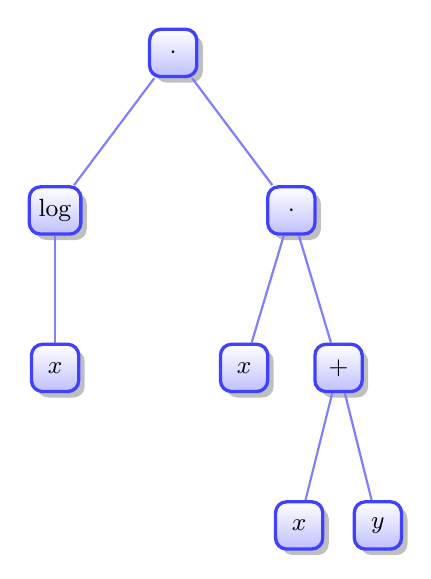
\begin{tikzpicture}
 		[font=\small, edge from parent, 
 		every node/.style={top color=white, bottom color=blue!25, 
 			rectangle,rounded corners, minimum size=6mm, draw=blue!75,
 			very thick, drop shadow, align=center},
 		edge from parent/.style={draw=blue!50,thick},
 		level 1/.style={sibling distance=3cm},
 		level 2/.style={sibling distance=1.2cm}, 
 		level 3/.style={sibling distance=1cm}, 
 		level distance=2cm,
 		]
 		\node (A) {$\cdot$} 
 		child { node (B) {$\log$}
 			%child { node {x} 
 				%edge from parent node[left=.5em,draw=none] {} }
 			child { node {$x$}}
 		}
 		child {node (C) {$\cdot$}
 			%child { node {x}
 				%	child { node {C1a}}
 				%}
 			child { node {$x$}}
 			child { node {$+$}
 				child { node {$x$}}
 				child { node {$y$} %edge from parent node[right=.5em,draw=none] {$\frac{a}{b}$}
 				}
 			}
 		};
 		%	child { node {+} 
 			%	child { node {2}}
 			%	child { node {$x$}}
 			%};
 		
 	\end{tikzpicture}
 	
 	\caption{Syntax tree representation for the expression $\log{x} \cdot   ( x \cdot ( x + y )˘)$}
 	\label{fig:syntax-tree-example}
 \end{figure}
 

\subsection{The \textsc{RILS}-\textsc{ROLS}  classifier}

In this section we first describe the basic components of the \textsc{Rils}-\textsc{Rols} algorithm, the main ingredient of the \textsc{Rils-Rols} classifier. For all the details on this method, we refer readers to the paper~\cite{kartelj2023rils}. 

 \textsc{Rils}-\textsc{Rols} combines the popular iterated local search meta-heuristic (ILS)~\cite{lourencco2003iterated,lourencco2010iterated} with the ordinary least square method (OLS)~\cite{leng2007ordinary}.  Iterated local search serves as a method backbone,  mainly tackling combinatorial aspects of the problem consisting of searching for essential functional forms of good model representations which are additionally tuned later in the search. OLS algorithm tackles continuous aspects of the problem, that is it efficiently determines best-fitting coefficients of  linear  combinations within solution equations. One of the  important steps of the algorithm is generating perturbations in the vicinity of a solution, i.e. the set of solutions  which are with a ``distance'' of 1 (called 1-perturbation). This is done by making simple changes on the \emph{per-node} level of solution's expression tree.  These per-node change operations are predefined in the algorithm, see more about it in~\cite{kartelj2023rils}. After generating the set of all such 1-perturbation trees representing solutions around solution $s$, first all of them are  simplified, and subsequently improved by local search procedure (explained below),  and then examined by calculating their fitness values (explained below). The one solution among them with the best fitness is compared to the fitness of the best-so-far known solution. Note that this is a modification in comparison to the original \textsc{Rils}-\textsc{Rols} implementation that only considers the first-improvement strategy among the set of all 1-perturbation around $s$, where the order of examination was according to their $R^2$ scores. If a new best solution has been found, it becomes a new incumbent ($s_{best}$) and $s=s_{best}$ or otherwise a random solution s' from the set of all 1-perturbations around $s_{best}$ is picked and the set of 1-perturbations are generated around $s'$. Afterwards, a random solution is picked from that set and stored as solution $s$ (representing a 2-perturbation of $s_{best}$) in the next iteration. It is worth mentioning that the algorithm only uses a piece of the data sampled from the input data for searching appropriate model  at each iteration. The size of the data increases (it becomes duplicated w.r.t. the data size of the previous iteration) once there is no improvement in the algorithms after a number of iterations. The algorithm iterates as long as none of the termination criteria are met: ($i$) the maximal running time has been reached; ($ii$) the maximal number of fitness calculations has been made.
  
 
 \textit{Fitness function}. To verify goodness of solutions in the search process, a carefully designed fitness function has been utilized that takes into consideration three model quality scores -- $R^2$, \emph{RMSE} and the size of model, combined into a non-linear function. It is of the following form:
 \begin{equation}\label{eq:fitness-rils-rols} 
 	 fit(s) = (1+ RMSE(s)) \cdot (2-R^2(s)) \cdot (1+ p_{size} \cdot |s|)
 \end{equation}
where  $p_{size}>0$ is a strategic parameter and $|s|$ is the size of solution (model) $s$ -- that is the number of nodes of its tree representation. 

  \emph{Local search}. In order to intensify the search, an efficient local search procedure has been employed around each solution based on a concept of the \emph{extended} 1--perturbations. That is,   solutions which are in the vicinity of $s$ are generated w.r.t.\ the extended set of pre-defined per-node-changes, see again~\cite{kartelj2023rils}.  LS applies the best-improvement search strategy.  Thanks to the extended  per-node-changes, the LS procedure additionally performed an efficient and  important general coefficient tuning, unlike OLS that does the fitting only in linear combinations.  In the context of fitness function \emph{fit}, an effective way of calculation is performed utilizing the \emph{expression caching}. 
 
 \emph{Rils-Rols classifier}.  Now, it is necessary to turn the \textsc{Rils}-\textsc{Rols} algorithm, a state-of-the-art tool for solving the Symbolic regression problem, into a classifier. We do it for the problem of (symbolic) binary classification w.r.t.\ the value of a treshold parameter. More precisely, for a model $s$ obtained by executing the \textsc{Rils}-\textsc{Rols} algorithm evaluated on the historical data $D$, the concrete $\textbf{x}_i \in D$ is mapped to the corresponding target value of 1 if $s(\textbf{x}_i) \geq treshold$ or 0 otherwise. Interestingly, according to our experimental evaluation, the best \textit{accuracy} is  obtained by setting $treshold=0.5$. 
  
 \subsection{The \textsc{Hroch}  classifier}
\textit{ The HROCH parameters}  %https://github.com/janoPig/HROCH/blob/main/docs/HROCH.md
 \begin{itemize}
 	\item $pop_{size}$: Number of individuals in the population
 	\item $pop_{sel}$:  the size of a tournament selection in each iteration (default value is equal to 4)
 	\item $feature_{probs}$: the probability that a mutation will select a feature
 \end{itemize}
 
\textit{ Stopping criteria}. The algorithm run until at least one of the two criteria is met:
 \begin{itemize}
 	\item  $time_{limit}$: time limit is reached
 	\item $iter_{limit}$: number of iteration has exceeded.
 	
 \end{itemize}
 The algorithm work on the set of predefined mathematical functions such as: pow, exp, log, sqrt, sin, cos, tan, asin, acos, atan, sinh, cosh, tanh. 
 The set of predefined arithmetic operators includes but not limited to: no use of operation, $+, -, \cdot, /,$ and sq2. Some other operations that may be used are the inverse, the multiplicative inverse, $\min, \max$, floor, ceil, $\geq, >, \leq, <$, etc. 
 
 Pre-defined values in the algorithm:
 
 \begin{itemize}
 	\item Predefined constants along with the probabilities of selecting one of the predefined constants used during initialization 
 	\item Predefined constants used during equations search along with the pre-defined probabilities of their selection
 \end{itemize}


\textit{Fitness function}.  TODO\\

\textit{Tournament selection}.  Among the current set of solutions (models), the $pop_{sel}$ if them is selected randomly and one with the best fitness score has been returned afterwards. 

\textit{Mutation}. TODO
 \fxnote{Marko: TODO -- the main algorithm's flow...} % https://github.com/janoPig/sr_core/tree/main/Hroch
 
 
 

 
\section{Experimental evaluation}\label{sec:experiments}

Our  algorithm is implemented in XX. All experiments concerning our method are conducted in the single-core mode, on a PC with Intel i9-9900KF CPU @3.6GHz, 64GB RAM, under Windows 10 Pro OS. The RAM consumption was very small (up to a few hundred megabytes).   

The following algorithms  are compared: XX...


\subsection{Datasets}
 XX
 
\section{Conclusions and future work}\label{sec:conclusions}
XX
 \fxnote{TODO}
\begin{backmatter}

 \section*{Acknowledgments}%% if any
Not applicable.

 \section*{Funding}%% if any
Not applicable.

%\section*{Abbreviations}%% if any
%Text for this section\ldots

  \section*{Availability of data and materials}%% if any
 All accompanying resources regarding this paper can be found in the GitHub repository \url{https://github.com/XX/XX}. 

\section*{Ethics approval and consent to participate}%% if any
Not applicable. 

\section*{Competing interests}
The authors declare  no competing interests.

\section*{Consent for publication}%% if any
Not applicable. 

\section*{Authors' contributions}
Both A.K. and M.Dj. contributed to the conception of the work. A.K. worked on the implementation of method and the design of experiments. M.Dj. worked on analysis and discussion of the results, introduction and literature review. 

%\section*{Authors' information}%% if any
%Text for this section\ldots

%%%%%%%%%%%%%%%%%%%%%%%%%%%%%%%%%%%%%%%%%%%%%%%%%%%%%%%%%%%%%
%%                  The Bibliography                       %%
%%                                                         %%
%%  Bmc_mathpys.bst  will be used to                       %%
%%  create a .BBL file for submission.                     %%
%%  After submission of the .TEX file,                     %%
%%  you will be prompted to submit your .BBL file.         %%
%%                                                         %%
%%                                                         %%
%%  Note that the displayed Bibliography will not          %%
%%  necessarily be rendered by Latex exactly as specified  %%
%%  in the online Instructions for Authors.                %%
%%                                                         %%
%%%%%%%%%%%%%%%%%%%%%%%%%%%%%%%%%%%%%%%%%%%%%%%%%%%%%%%%%%%%%

% if your bibliography is in bibtex format, use those commands:
\bibliographystyle{bmc-mathphys} % Style BST file (bmc-mathphys, vancouver, spbasic).
\bibliography{bib}      % Bibliography file (usually '*.bib' )
 
 

%%%%%%%%%%%%%%%%%%%%%%%%%%%%%%%%%%%
%%                               %%
%% Figures                       %%
%%                               %%
%% NB: this is for captions and  %%
%% Titles. All graphics must be  %%
%% submitted separately and NOT  %%
%% included in the Tex document  %%
%%                               %%
%%%%%%%%%%%%%%%%%%%%%%%%%%%%%%%%%%%

%%
%% Do not use \listoffigures as most will included as separate files
 

 
 

%\section*{Additional Files}
%  \subsection*{Additional file 1 --- Sample additional file title}
 %   Additional file descriptions text (including details of how to
 %   view the file, if it is in a non-standard format or the file extension).  This might
 %   refer to a multi-page table or a figure...
 

\end{backmatter}
\end{document}
